\begin{figure*}[!t]
\centering
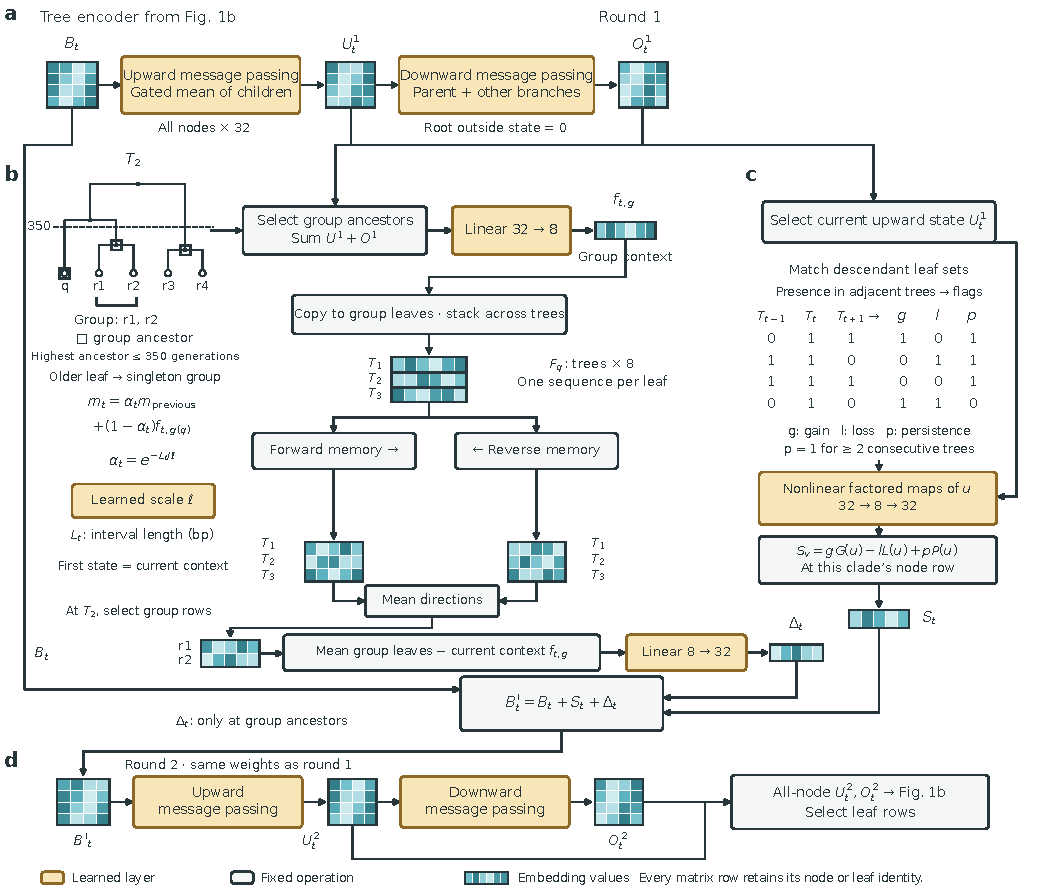
\includegraphics[width=\textwidth]{figures/TreeLoom_encoder.pdf}
\caption{Expansion of the tree encoder in Figure~\ref{fig:architecture}b.
\textbf{a,} A complete upward traversal produces $U^1$, followed by a downward traversal producing $O^1$. Rows retain node identities. Upward state $U$ corresponds to $h$ in the equations.
\textbf{b,} Each leaf joins the group represented by its highest ancestor no older than 350 generations. Older samples remain singleton groups. A projection of the representative's summed states gives the group context $f$, copied to its leaves. Separate histories follow each leaf across trees, even when its group changes. Forward and reverse exponential memories are averaged per leaf and then over the current group's leaves. Subtracting the current context and projecting gives a correction $\Delta$, added only at group representatives. The $T_2$ example is repeated at every interval. Here $m,\alpha,L,\ell$ correspond to $z,\rho,w,\lambda$ in the text.
\textbf{c,} Exact descendant sets determine gain, loss and persistence flags for proper clades. These flags may overlap. Learned factored maps $G,L,P$ transform the current upward state and place correction $S$ at its clade representative. Their equations appear in the supplement.
\textbf{d,} Both corrections enter the original base before the second complete upward and downward round, which reuses the first round's weights. Both all-node outputs return to leaf selection in Figure~\ref{fig:architecture}b.}
\label{fig:encoder}
\end{figure*}
